\documentclass[a4paper,11pt,fleqn]{article}
\usepackage{amssymb}
\usepackage[polish]{babel}
\usepackage[cp1250]{inputenc} %1250
\usepackage[T1]{fontenc}
\usepackage{graphicx}
\usepackage{anysize}
\usepackage{enumerate}
\usepackage{times}
\usepackage{subfig}
\usepackage{hyperref}
\hypersetup{colorlinks = true, allcolors = blue}
\usepackage{graphicx} 

%latech wikibooks floatfigures, pakiet wrapfig i do ramek framed
%to diam ma byz zwykla czcionka ale w trybie matematycznym
%\marginsize{left}{right}{top}{bottom}
\marginsize{2cm}{3cm}{3cm}{3cm}
\sloppy

\begin{document}

\section*{Ca�ka Riemanna}
Niech dana b�dzie \href{https://pl.wikipedia.org/wiki/Funkcja_ograniczona}{funkcja ograniczona} $f\!\colon[a,b]\to\mathbb{R}$. \emph{Suma cz�sciowa} (Riemanna) nazywa si� liczb� 
\[
R_{f,P(q_{1},\dots,q_{n})}=\sum_{i=1}^{n}{f(q_{i})\cdot\Delta{p_{i}}}.
\] 
Funkcj� $f$ nazywa si� \emph{ca�kowaln� w sensie Riemanna} lub kr�tko \emph{R-ca�kowaln�}, je�li dla dowolnego ci�gu normalnego $(P^k)$ podzia��w przedzia�u $[a,b],$ istnieje (niezale�na od wyboru punkt�w po�rednich) granica
\[
R_f=\lim_{k \rightarrow \infty}{R_{f,P^{k}(q_{1}^{k},...,q_{n}^{k})}}
\]
nazywana wtedy \textbf{ca�k� Riemanna} tej funkcji.~R�wnowa�nie:~je�eli istnieje taka liczba $R_{f},$ �e dla dowolnej liczby rzeczywistej $\varepsilon >0$ istnieje taka liczba rzeczywista $\delta >0,$ �e dla dowolnego podzia�u $P(q_{1},\dots ,q_{n})$ o �rednicy ${diam}\;P(q_{1},\dots ,q_{n})<\delta $ b�d� te� w j�zyku rozdrobnie�:~�e dla dowolnej liczby rzeczywistej $\varepsilon >0$ istnieje taki podzia� $ S(t_{1},\dots ,t_{m})$ przedzia�u $[a,b],$ �e dla ka�dego podzia�u $P(q_{1},\dots ,q_{n})$ rozdrabniaj�cego $S(t_{1},\dots ,t_{m})$ zachodzi
\[
\left|R_{{f,P(q_{1},\dots ,q_{n})}}-R_{f}\right|<\varepsilon .
\]
Funkcj� $f$ nazywa si� wtedy ca�kowaln� w sensie Riemanna (R-ca�kowaln�), a liczb� $R_{f}$ jej ca�k� Riemanna.

\begin{figure}[!htb]
\centering
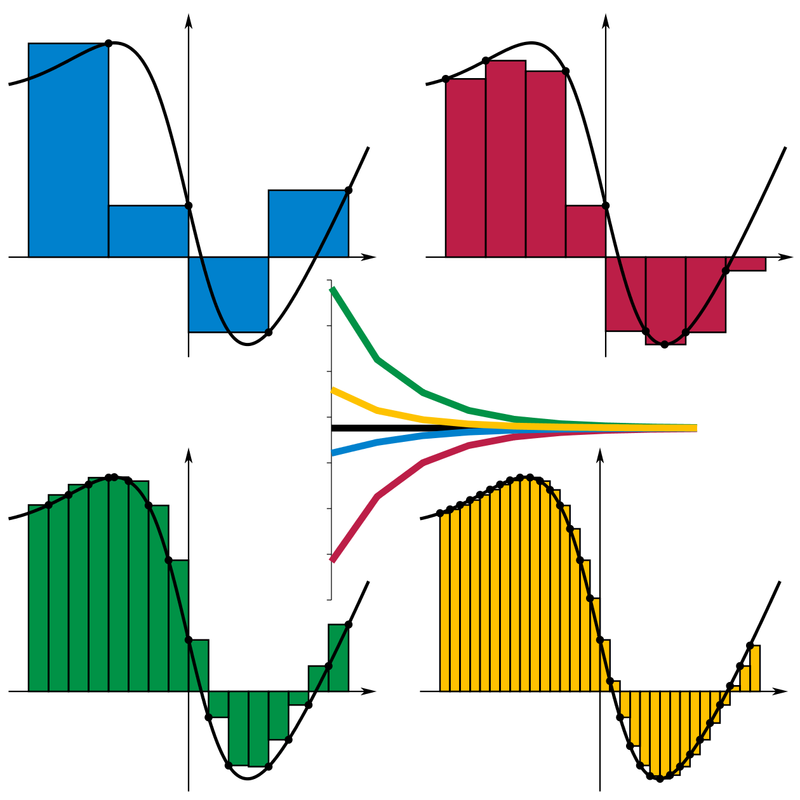
\includegraphics[width=3cm]{800px-Riemann_sum_convergence.png}
\caption{obraz}
\label{fig:obrazek k}
\end{figure}

\end{document}
